\subsection{Xem thông tin người dùng}
\subsubsection{Sơ đồ use-case}
\begin{figure}[H]
    \centering
    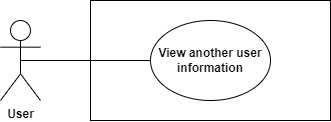
\includegraphics[width=0.55\textwidth]{Images/UseCase/User.png}
    \caption{Sơ đồ use-case cho chức năng xem thông tin người dùng}
\end{figure}
\newpage
\subsubsection{Đặc tả use-case cho chức năng xem thông tin người dùng}
\begin{center}
    \arrayrulecolor{cyan!75!black}
    \arrayrulewidth=2pt
    \begin{longtable}{
        |>{\raggedright\arraybackslash}p{3cm}
        |>{\raggedright\arraybackslash}p{13cm}
        |}
        \hline
        \rowcolor{cyan!75!black} \textcolor{white}{\textbf{Use-case name}} & \textcolor{white}{\textbf{XEM THÔNG TIN NGƯỜI DÙNG}}
        \\\hline
        \rowcolor{cyan!10!white} \textit{Actor} & Người dùng
        \\\hdashline
        \rowcolor{cyan!10!white} \textit{Description} & Tính năng cho phép người dùng xem thông tin cá nhân của người dùng khác.
        \\\hdashline
        \rowcolor{cyan!10!white} \textit{Preconditions} & Không có
        \\\hdashline
        \rowcolor{cyan!10!white} \textit{Postconditions} & Thông tin cá nhân của người dùng khác được hiển thị trên giao diện ứng dụng.
        \\\hdashline
        \rowcolor{cyan!10!white} \textit{Trigger} & Người dùng chọn vào tên của người dùng đó trên ứng dụng, có thể được hiển thị ở mục bài đăng tải, bình luận cũng như phản hồi.
        \\\hdashline
        \rowcolor{cyan!10!white} \textit{Main flow} &
        1. Ứng dụng hiển thị thông tin của người dùng khác trên giao diện. \newline
        2. Người dùng có thể theo dõi các thông tin cá nhân như tên, hình ảnh đại diện, email, số điện thoại...
        \\\hdashline
        \rowcolor{cyan!10!white} \textit{Alternative flow} & Không có
        \\\hdashline
        \rowcolor{cyan!10!white} \textit{Exception flow} &
        \textbf{Nếu ứng dụng gặp lỗi khi hiển thị thông tin của người dùng khác, ứng dụng thông báo lỗi và yêu cầu người dùng thử lại sau} \newline
        1a.1. Ứng dụng hiện lỗi khi hiển thị thông tin của người dùng khác. \newline
        1a.2. Ứng dụng thông báo yêu cầu người dùng thử lại sau.
        \\\hline
        \caption{Đặc tả use-case cho chức năng xem thông tin người dùng}
    \end{longtable}
\end{center}
